\section{Parte di statistica descrittiva}
In questa fase preliminare si illustreranno le principali considerazioni fatte sul dataset fornito.
\subsection{Boxplot dei dati}
Si considerino i seguenti boxplot delle variabili del dataset.
\begin{figure}[h]
	\centering
	\subfigure[Boxplot della variabile dipendente y\_VideoQuality]{
		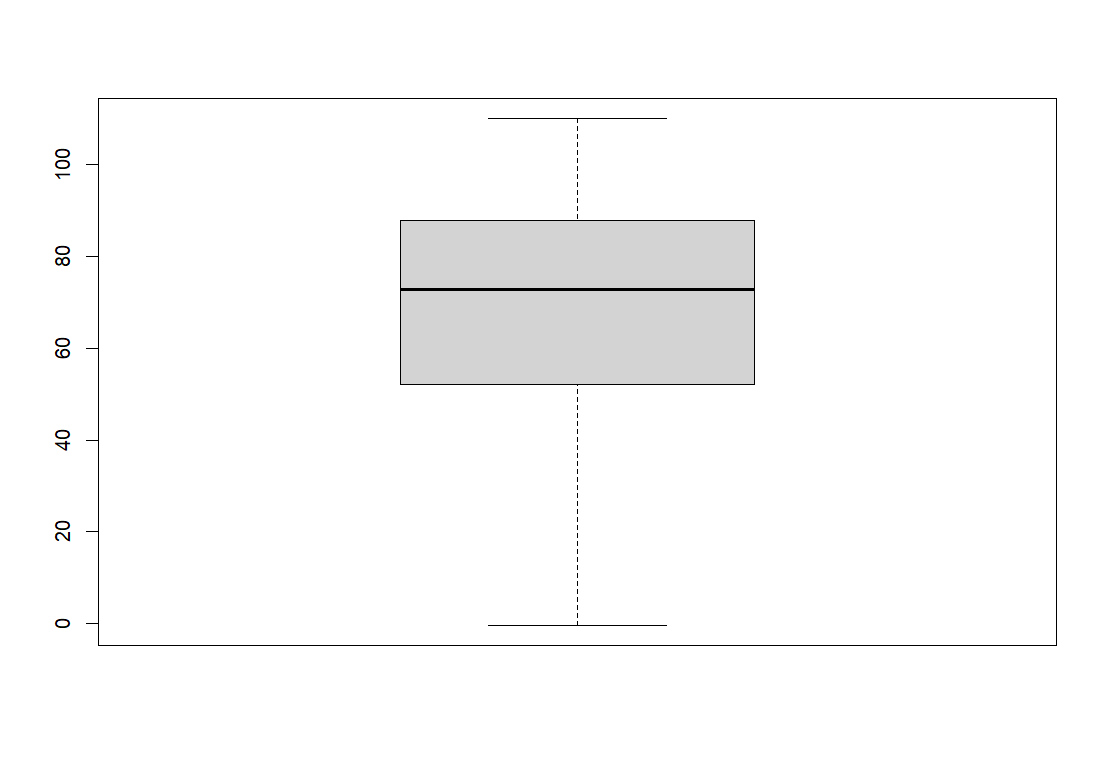
\includegraphics[width=0.65\linewidth]{../graphs/DescriptiveStatisticPlots/boxplot_y_VideoQuality}
		\label{fig:boxplotyvideoquality}
	}
	\hfill
	\subfigure[Boxplot delle variabili indipendenti x\_i]{
		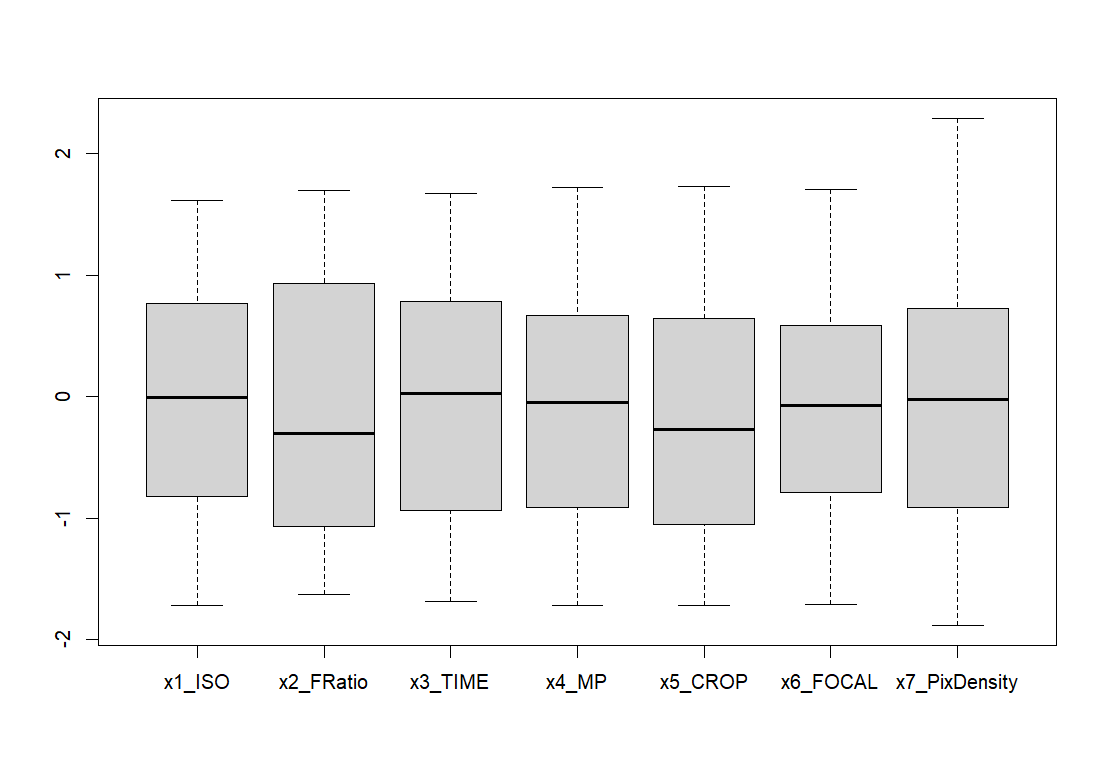
\includegraphics[width=0.65\linewidth]{../graphs/DescriptiveStatisticPlots/boxplot_all_x_i}
		\label{fig:boxplotallxi}
	}
	\caption{Boxplot delle variabili considerate}
\end{figure}

Si osservi innanzitutto che i valori per ciascuna variabile sono tutti contenuti all'interno dell'intervallo interquartile e che quindi non sono presenti outliers. Per quel che riguarda la variabile 


\subsection{Analisi di correlazione}
